% This example An LaTeX document showing how to use the l3proj class to
% write your report. Use pdflatex and bibtex to process the file, creating 
% a PDF file as output (there is no need to use dvips when using pdflatex).

% Modified 

\documentclass{l3proj}
\begin{document}
\title{A Website Translation Service}
\author{Alasdair Campbell \\
	Andrei Mustata \\
	Paul Moore \\
        Stephen Hayton \\
	Wei Zhang}
\date{9th February 2012}
\maketitle
\begin{abstract}

Since the writing of the earliest manuscripts and documents there has been a need for translation so that the people of the world could understand what had been written or said, in their own native language. Translation is just as relevant today as it was thousands of years ago, although the processes have modernised considerably. The focus of this project is to create an online presence and document delivery system for a Glasgow based translator who is creating her own document translation business. Our goal is to improve upon the translation sites currently available and to give a unique, modern and fresh feel to translation.

\end{abstract}
\educationalconsent
\tableofcontents
%==============================================================================
\chapter{Introduction}
\label{intro}
\textit{\small{This article assumes a basic general computing knowledge from the reader. If any words or phrases are not understood, consult the glossary of terms (Section~\ref{sec:gloss}) at the end of the document. All content is owned by the authors of this document or is otherwise referenced in bibliography (Section~\ref{sec:bibl})}}\\
\section{Background}
As part of our degree in third year we are tasked with a team project. This relates to computing disciplines new to us and draws on knowledge gained from the preceding two years at University. Teams were randomly assembled at the beginning of semester and our team received the project to create a website providing a document translation service for a real client. It was a pleasing allocation mainly due to the latter part of the task: the fact we would be working with a real client. This bespoke web-based service builds on our client's existing business model, with the specific aims to bring about an expansion in her company, while also facilitating an improvement to her working practice as a whole.\\
\\
There are many translation services available on the Internet already, a simple Google search for online translation returns around one hundred and fifty nine million results. We have looked into various different types of translation and interpretation websites during our research and have found pros and cons from each. This vast number of already available websites creates a desire of competing with what's already available, by trying to improve areas where other websites have fallen short. We believe one of the key factors that makes a modern website successful is minimalistic design: it offers simple and effective functionality and is aesthetically pleasing. The combination of these things means users are more likely to use the website after stumbling across it in a search, perhaps, and will ultimately give our client a larger customer base. To clarify, we are not trying to re-invent the wheel with our project. We have used frameworks and other free source components in the development of our website. The system is mainly built around the LAMP structure, i.e., Linux + Apache + MySQL + PHP. We believed that these choices would lower the costs of an eventual upgrade of the system, as opposed to having used some more exotic technologies that come at the cost of losing the robustness and stability that we needed. We aimed to maintain a user friendly feel and look and believe that is something we accomplished well. One of the things that encourages this notion is the fact we have created a simple 3-stage process in which users can register, upload documents, and request languages to translate to.\\ 
\section{Aims}
To briefly summarise our task at hand: we are to develop a website for a free-lance translator. It should allow users to upload documents, request one of the available languages to translate to, and submit a request for translation. Our client should then be able to review those submitted documents and send a quote to the user for the job to be translated. If happy, the user should then be able to pay for the job(s) via Paypal, and then receive their translated document after a period of time. Additional required features of the website will be discussed later. Listed below are a few important points on why using a software system to manage documents and to keep track of discussions and tasks has advantages over the current system. It also serves as a rough timeline of the clients activity:

\begin{itemize}
	\item
	makes {\bf planning} deadlines easier, since computers are better than humans
	at taking large amounts of data and comparing, adding, etc.;
	\item
	makes {\bf file managing} easier;
	\item
	improves {\bf productivity} - now that the other two are out of the way, the
	user of the system has more time to think of things that matter more.
\end{itemize}

By having all the job details clearly stated and planned, the clients are encouraged to pay more attention and to take it more seriously. It also introduces the notion of accountability on both sides - client and translator. Having a detailed log of all the documents delivered to which clients and when, would make keeping track of the activity easier to do. By using an electronic payment system, the risk of having unpaid jobs is greatly reduced. It also gives the business a more professional look and makes our client less vulnerable to hacking attacks as opposed to other methods of payment.\\
\section{Motivation}
An essential part of our requirements gathering process was the first meeting with our client, Joelle Cimatche. Our team had been forewarned by our supervisor that the client was not very "technically minded", so we tried our best to prepare questions that did not assume she had much experience with a computer. It's fair to say that after reading the initial brief for the project we made assumptions as to the needs of the client, addressing the problem from our viewpoint. Realising we should expect to review these assumptions during the process of working on the requirements capture is a valuable lesson for future employment. Working with an individual or organization, firmly on the periphery of Internet technology adds it's own challenges, particularly during the requirements capturing process. At the meeting, the client explained she had a very basic understanding of word processing applications and the Internet, and not much else. This presented us with an additional challenge. We couldn't simply relay technical jargon to the client and expect her to provide useful feedback. Not only that, our team would have to create a very easy-to-use admin end to the website that she could learn quickly. As we advanced the development of the website, we would have to be very clear and straightforward when updating her on our progress.  \textbf{Figure 1.1} somewhat illustrates the challenge we have. It is basically the "adoption rate curve" for a percentage of users of new technologies. In other words, how quickly users can say they understand a new technology after it is first released. It is known as Roger's bell curve. Our client would be at the far thright end of the spectrum, in the 16\% of users described as "Laggards" in the graph.\\
	
\begin{figure}
\begin{center}
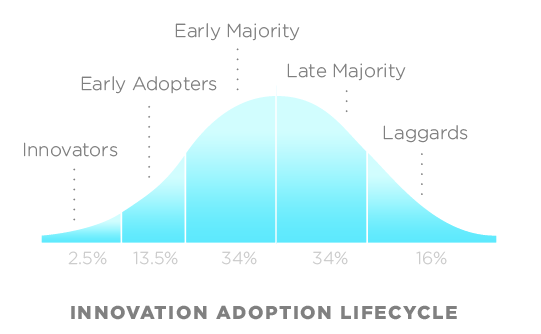
\includegraphics[scale=0.6]{DiffusionOfInnovation}
\caption{Roger's bell curve, source: http://en.wikipedia.org/wiki/File:DiffusionOfInnovation.png}
\end{center}
\end{figure}
	
Reflecting on our experiences in our project, working with the client has not been exceptionally easy. One of our main challenges is that our client is a novice computer user. Quite ironically, it has been a task for us to translate regular computing jargon into layman's terms in order for them to understand. This was critical in our requirement gathering process. In spite of this additional challenge that teams working with other projects might not particularly face, it is not necessarily something that is discouraging for us. When we eventually graduate and face real world software projects, it won't always be technically minded people like ourselves we deal with, it will people who are more similar to our client. It will provide us something to drawn upon when we are asked to recount our experiences in future interviews. The opportunity to work with a real client will serve us as great preparation for working life.\\
\\
Our project lives on the Internet. Ten years ago, the Internet was everywhere, but now it's even more so. It's a rapidly evolving area where new technologies and new techniques are developed very quickly. These have been made easy to use by anyone, regardless of: computer knowledge, nature of their device (mobile or desktop) or their operating system. All they need is an up-to-date web browser - arguably an easy requirement to fulfill, since most of them update automatically. So, there is a large audience that our project can reach, and that is considerably motivating for everyone in our team who worked on this project.\\

\section{Preliminaries}
To understand this report it is necessary to understand that we do not have to implement a translation algorithm. We are providing customers with an interface to send documents to be translated by a professional translator for a fee, and then returned in the chosen translated language using the same web interface. To understand the process that we have devised it would be advantageous to have a simple understanding of how a database works. As mentioned earlier, we have adopted several frameworks in our project development. These include Bootstrap (CSS, HTML), CodeIgniter and phpMyAdmin (all of which are discussed in Section~\ref{chap:design} later). These frameworks provide advanced functionality which will, in most instances, not be necessary for our project and will not be utilised. Conversely, it allows us to demonstrate that we are professional software developers and that we are capable of software re-use.

\section{Outline}
The remainder of this report will go into more detail on the background research of our project, expand on our motivation and set out our group organisation and project plan. After this we will detail our design ideas and methodologies, before moving on to document our implementation, testing and evaluation. We will then discuss any problems encountered and the results of our evaluation before revealing the final status of the project, giving a detailed outline of the deployed site including any graphics and information relating to Bethel Translations.
 

%==============================================================================
\chapter{Design}
\label{chap:design}
\section{Requirements Gathering}

At the beginning of our project we met with our client and our project supervisor to discuss her requirements. Our client currently translates for an agency and is looking to create her own translation business. To this extent she wishes to have a website built to allow her to gain an online presence in translation and to digitize the process of receiving and sending translations. We were armed with a long list of questions and ideas for the meeting and a transcript is included as an appendix. \\
\\
As software developers naturally would when creating anything from scratch, our team looked for similar websites already in existence. We identified common useful features of each, and also those features that were not so useful, and listed some we thought could be useful but simply did not exist in any of the sites we examined. One recurring theme we noticed in a majority of similar translation websites was that the home page was very cluttered and full of text. In other words, the process that the user had to follow to obtain some translation of a document was not extremely clear. Instead, they were met with various registration options, other services and annoying advertisements. From previous modules in our degree, namely IM2 and IS3, our team had experience of applying Jakob Nielsen's heuristics to obtain a successful user interface. We wanted to develop the idea that our website would display the minimal amount of information to a user by providing the registration, document upload and language selection elements on a single page, in a simple 3 step process. Our interface would then fall in line with the principle that user interfaces should have an aesthetic and minimalist design. \footnote{http://www.useit.com/papers/heuristic/heuristic\_list.html} We believe this is an extremely important aspect of any modern website based on the way that users make a decision of whether or not to use the services offered by the website. For example, imagine a user enters a Google search for "Translation service" and clicks our website in the results page. If the page they are met with looks too complicated or confusing in nature, the user simply clicks "Back" on their web browser, and goes to the next appropriate web page. If however the website looks clean, simple, and easy to use, the user would be more inclined to use it properly. We believe that our 3-step process found on the home page encourages anyone that requires a translation service for the provided languages to at least try for a quote, if not go through with the whole process.\\
\\
With this approach in mind, we began to create some wireframes in order to form a solid idea of how this 3-stage process would physically look on our website. \textbf{Figure 2.1} illustrates our early attempt at doing so.

\begin{figure}
\begin{center}
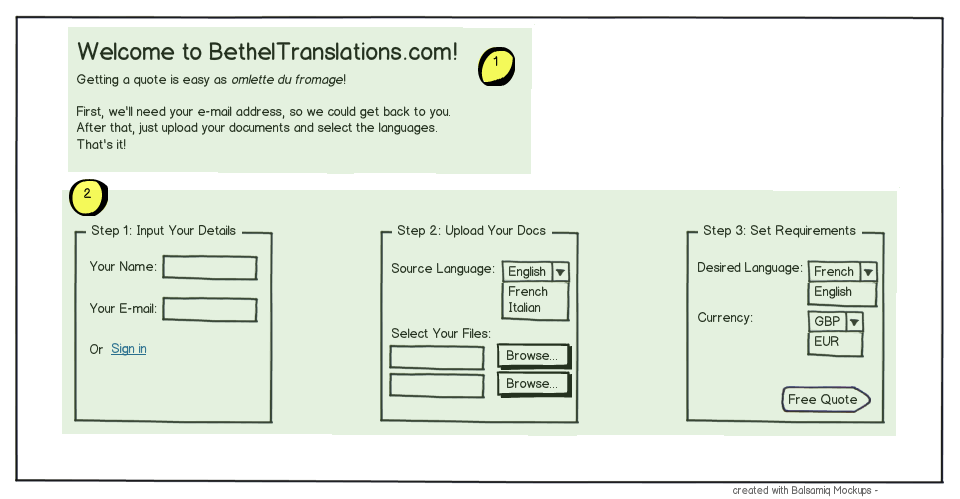
\includegraphics[width=\linewidth]{wireframes/bt-3step}
\caption{The 3-step process}
\end{center}
\end{figure}

The layout is intuitive, flowing and simple to approach. In this early design we have split the page into two sections. In section 1 the user is presented with a short amount of precise text detailing the main function of the site. Subsequently, in Section 2 the user simply enters some details, adds the documents, sets the requirements and clicks a button to request a quote. \\There is no daunting, large form based entry that some other websites encapsulate. It is minimal and it is undemanding of users. Obviously, the majority of the work done by our system would be when the user clicks "Get your quote", and the system would have to register a user (pending email validation), upload their documents to the file store, associate a jobid and requirements, and place the job in our client's pending work queue. The implementation of such functions are discussed later in Section~\ref{chap:impl}.\\
\\


\section{User Process}
With this 3 stage process as our main design factor of the website, we began to consider the main user groups of the website. We identified the needs of two main user classes: the \textbf{clients} and the \textbf{translator}

The clients are the users of the service, the visitors of the website. However, as far as the system is concerned, not all visitors are clients, because, in order for a visitor to become a client, he must register with the service. So we decided to have a visitor as a category with a registered user a subcategory. A registered user would then possess all the same abilities as a visitor with some specialised capabilities:

\textbf{Visitor}
\begin{itemize}
\item{Rationale: The visitor is just visiting. An anonymous visitor of the website.}
\item{Background: "I need to get some documents translated. I came across this website and before I register or send any of my documents, I want to make sure that I'm€™m dealing with a serious service."}
\item{He is a potential client, therefore the steps which he must make in order to become one must be as clear as possible.}
\item{His \textbf{goal} is to inform himself about the service. In order for him to be converted, he must be convinced that the service provided is of great quality, so the system's€™s goal is to make itself trustworthy. Also, a clear privacy policy regarding e-mail addresses and the documents should be available, since they might contain sensitive data.}
\end{itemize}
\textbf{Client}
\begin{itemize}
\item{Rationale: The client is a registered user of the system.}
\item{He has the same goals as the visitor, but, now that he is registered, he trusts the service a bit more. He has access to all the documents that he ever submitted for translation and can view each of the \textbf{job statuses} for which his documents are contained within. He can view documents he has paid for, and up to a certain period of time, download both the original copy and the translated copy. He can also view some other useful statistics on his previous jobs.}
\end{itemize}
\textbf{Administrator/Translator}
\begin{itemize}
\item{Rationale: The translator is the one answering all the translation requests.}
\item{"As a translator, I must review the documents that my clients send me and quote them. After that, I must also translate them and let them know that I finished work."}
\item{His goal is to answer to all of the client's€™s requests, i.e. to quote By having all the details clearly stated and planned, the clients are encouraged
to pay more attention and to take it more seriously. It also makes both sides
- client and translator - more accountable.

Having a detailed log of all the documents delivered to which clients and when,
would make keeping track of the activity easier to do.

By using an electronic payment system, the risk of having unpaid jobs is greatly
reduced. It also gives the business a more professional look.the documents that are received and then translate them and send them back to them.}
\end{itemize}
Building upon the needs of these user classes, we needed to design a flexible system that provided functionality for all of these goals. Our main focal point would be the transition of \textbf{jobs}. In the context of our system, a job is what the website creates when the user uploads one or more documents for translation. Clients (registered users) would submit and pay for them. The translator would review them, download them and upload them. We considered the transition of jobs throughout the life cycle of a translation, as job statuses, and produced a sequence that is illustrated in \textbf{Figure 2.2}. 

\begin{figure}
\begin{center}
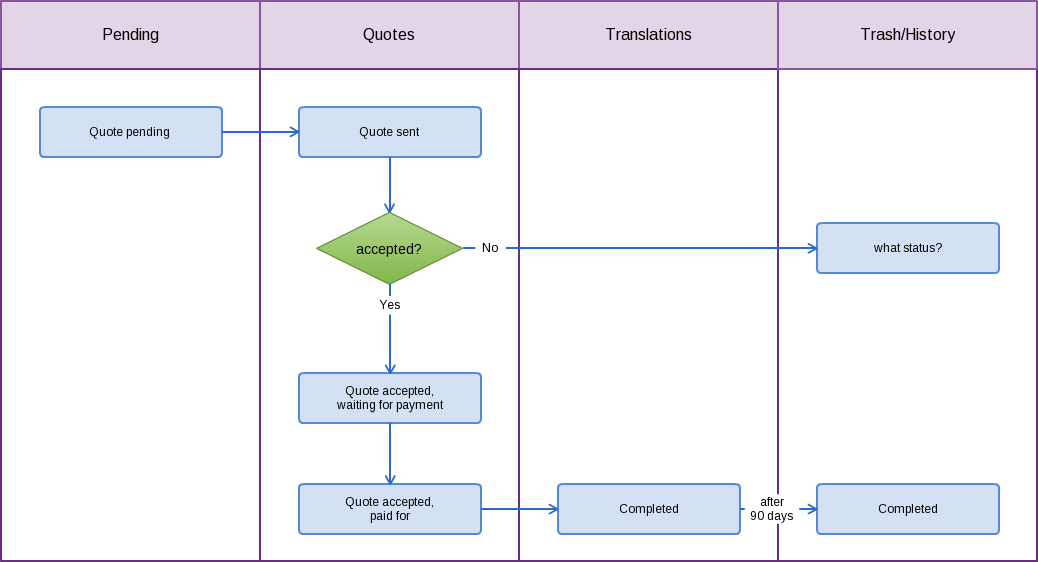
\includegraphics[width=\linewidth]{jobstatuses}
\caption{The transition of jobs through "statuses"}
\end{center}
\end{figure}

The diagram is much self-explanatory, but to summarise: Jobs that are submitted by the clients are placed in a \textbf{pending} work queue. The translator is able to review these documents and send some quote to the client. After a job has been quoted, it is placed in the \textbf{Quotes} queue. Quoted jobs are held in this queue until they are paid for via Paypal. When this has happened, they are moved to \textbf{Translations}, which is a breakdown of completed jobs. After a period of 90 days, jobs from this section are moved to \textbf{History} in order to reduce space on the server.

The transformation from this design plan to a viable user interface that is built upon these job statuses is described later in Section~\ref{chap:ui}.

\section{System Design and Wireframes}
After laying out the process of the website we focused on creating wireframe designs. 

\subsection{Template and Main Page}
From our earlier decision of creating a simple three step process and implementing this on our homepage, we took our wireframe and refined it to come up with the  \textbf{Main Template}.

\begin{figure}[ht]
\label{fig:The Main Template}
\begin{center}
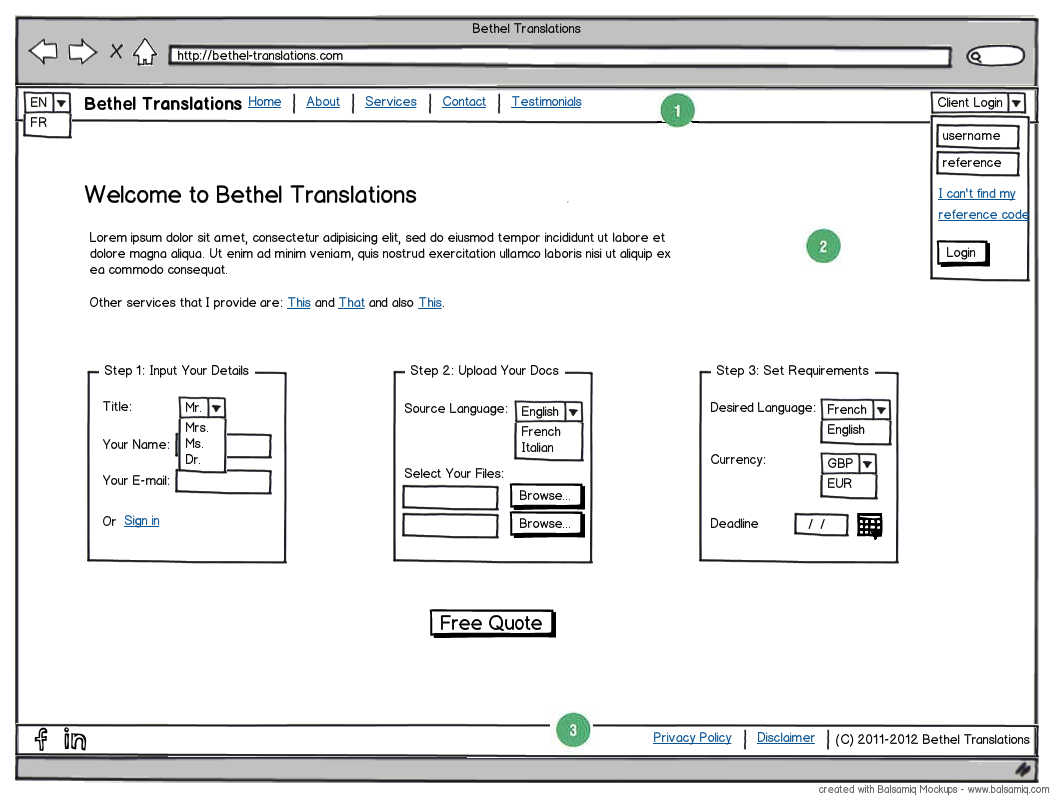
\includegraphics[width=\linewidth]{wireframes/bt-homepagev3}
\caption{The Main Template}
\end{center}
\end{figure}

The site-wide header (labelled 1) and footer (labelled 3) can clearly be seen to be simple and uncluttered.

%==============================================================================
\chapter{Implementation}
\label{chap:impl}

In this chapter, we describe how we the implemented the system from our design plan and the technologies used in doing so.


%------------------------------------------------------------------------------
\section{User Interface}
\label{chap:ui}
TBC

% - - - - - - - - - - - - - - - - - - - - - - - - - - - - - - - - - - - - - - -
%%\subsection{TBC - think project specific chapter}

%%TBC

%------------------------------------------------------------------------------
\section{Database Model}

Our database structure was designed after we had thoroughly revised our user registration and job transition processes. We envisaged there being four separate entities: one for \textbf{users} to become registered, one to represent \textbf{documents} being submitted, another for the \textbf{jobs} that are comprised of submitted documents and finally one for the documents once they have been \textbf{translated}. The attributes of each of these entities and the relationships between them is illustrated in \textbf{Figure 3.1} 

\begin{figure}
\begin{center}
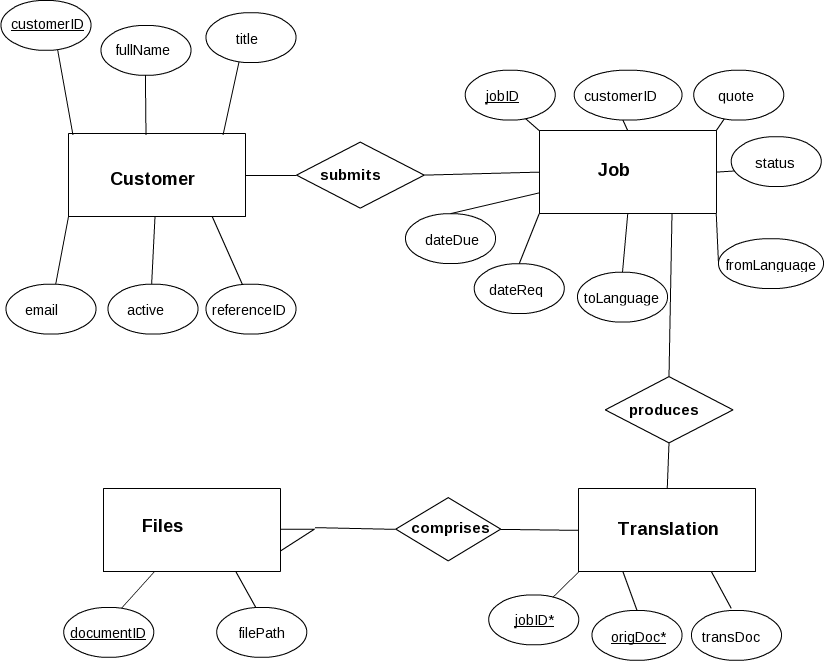
\includegraphics[width=\linewidth]{bt-dbstruct}
\caption{ER Diagram for Bethel Translations}
\end{center}
\end{figure}

The majority of activity for these tables occurs in the first three entities, as they are all populated in some way during the 3 stage process discussed earlier.

%==============================================================================
\chapter{Evaluation}

First feedback with Karen incl wireframes etc - Jan 25\\
Second feedback session with Karen incl more complete website design - Feb 9th

%==============================================================================
\chapter{Conclusion}

Team photo goes here? :)
A great project! etc..

%==============================================================================
\section{Contributions}

Alasdair done this...
Andrei handled that...
Stephen took responsibility for... 
Paul mainly done...
Wei was responsible for...	

%==============================================================================
\section{Appendices}
\subsection{Appendix A - Bibliography}
\label{sec:bibl}


\subsection{Appendix B - Glossary of Terms}
\label{sec:gloss}


\begin{itemize}
\item{\textbf{Free-lance} - Working for different companies at different times rather than being permanently employed by one company.} 
\item{\textbf{Client} - A person or organization using the services of a professional person or company.} 
\item{\textbf{Users} - A set of people who use or operate something, esp. a computer or other machine.}
\item{\textbf{Requirement gathering} - Determining the needs of a client through any form of communication.}
\item{\textbf{Software project} - Using the surrounding context, a software project aims to create application(s) using programming language(s) by adhering to project management principles.}
\item{\textbf{Programming language} - A programming language is an artificial language designed to express computations that can be performed by a computer.}
\item{\textbf{Web scripting language (\textit{PHP, Javascript})} - A scripting language is a programming language that allows control of one or more applications.}
\item{\textbf{Website development} - The process of constructing and maintaining a website.}
\item{\textbf{LAMP} - LAMP, (Linux, Apache, MySQL and PHP), is an acronym for a solution stack of free, open source software}
\item{\textbf{Web application framework} - A software framework that is designed to support the development of dynamic websites }
\item{\textbf{Open source} - Computer software for which the code is freely available }
\end{itemize}
%==============================================================================
\bibliographystyle{plain}
\bibliography{example}
\end{document}
